\begin{minipage}{0.75\linewidth}
\begin{figure}[h]
    \centering
    \begin{adjustbox}{max width=1.0\linewidth, keepaspectratio}
        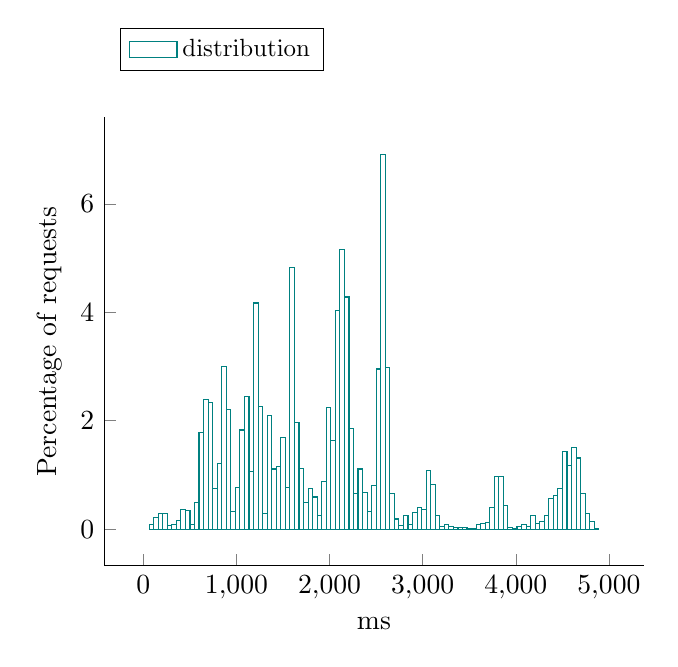
\begin{tikzpicture}
            \begin{axis}[ylabel = Percentage of requests, 
xlabel = ms, 
legend style = {nodes={scale=0.9, transform shape}, at={(0.03,1.2)}, anchor=north west, draw=black, fill=white, align=left, legend columns=3},
area style, mark size = 0pt,
 cycle list name = exotic,
  axis lines* = left]
		\addplot +[ybar interval] coordinates {
			 (62, 0.09375)
			 (110.78, 0.21875)
			 (159.56, 0.28125)
			 (208.34, 0.28125)
			 (257.12, 0.0625)
			 (305.9, 0.078125)
			 (354.68, 0.15625)
			 (403.46, 0.359375)
			 (452.24, 0.34375)
			 (501.02, 0.078125)
			 (549.8, 0.484375)
			 (598.58, 1.78125)
			 (647.36, 2.39062)
			 (696.14, 2.32812)
			 (744.92, 0.75)
			 (793.7, 1.20312)
			 (842.48, 3)
			 (891.26, 2.20312)
			 (940.04, 0.328125)
			 (988.82, 0.765625)
			 (1037.6, 1.82812)
			 (1086.38, 2.45312)
			 (1135.16, 1.0625)
			 (1183.94, 4.17188)
			 (1232.72, 2.26562)
			 (1281.5, 0.296875)
			 (1330.28, 2.09375)
			 (1379.06, 1.10938)
			 (1427.84, 1.15625)
			 (1476.62, 1.6875)
			 (1525.4, 0.765625)
			 (1574.18, 4.82812)
			 (1622.96, 1.96875)
			 (1671.74, 1.125)
			 (1720.52, 0.484375)
			 (1769.3, 0.75)
			 (1818.08, 0.59375)
			 (1866.86, 0.25)
			 (1915.64, 0.875)
			 (1964.42, 2.25)
			 (2013.2, 1.64062)
			 (2061.98, 4.03125)
			 (2110.76, 5.15625)
			 (2159.54, 4.28125)
			 (2208.32, 1.85938)
			 (2257.1, 0.65625)
			 (2305.88, 1.10938)
			 (2354.66, 0.671875)
			 (2403.44, 0.328125)
			 (2452.22, 0.8125)
			 (2501, 2.95312)
			 (2549.78, 6.90625)
			 (2598.56, 2.98438)
			 (2647.34, 0.65625)
			 (2696.12, 0.1875)
			 (2744.9, 0.0625)
			 (2793.68, 0.25)
			 (2842.46, 0.09375)
			 (2891.24, 0.3125)
			 (2940.02, 0.40625)
			 (2988.8, 0.359375)
			 (3037.58, 1.07812)
			 (3086.36, 0.828125)
			 (3135.14, 0.25)
			 (3183.92, 0.046875)
			 (3232.7, 0.078125)
			 (3281.48, 0.046875)
			 (3330.26, 0.03125)
			 (3379.04, 0.03125)
			 (3427.82, 0.03125)
			 (3476.6, 0.015625)
			 (3525.38, 0.015625)
			 (3574.16, 0.078125)
			 (3622.94, 0.109375)
			 (3671.72, 0.125)
			 (3720.5, 0.40625)
			 (3769.28, 0.96875)
			 (3818.06, 0.96875)
			 (3866.84, 0.4375)
			 (3915.62, 0.03125)
			 (3964.4, 0.015625)
			 (4013.18, 0.046875)
			 (4061.96, 0.09375)
			 (4110.74, 0.046875)
			 (4159.52, 0.25)
			 (4208.3, 0.109375)
			 (4257.08, 0.140625)
			 (4305.86, 0.25)
			 (4354.64, 0.5625)
			 (4403.42, 0.625)
			 (4452.2, 0.75)
			 (4500.98, 1.4375)
			 (4549.76, 1.17188)
			 (4598.54, 1.5)
			 (4647.32, 1.3125)
			 (4696.1, 0.65625)
			 (4744.88, 0.296875)
			 (4793.66, 0.140625)
			 (4842.44, 0.015625)
			 (4891.22, 0.0625)
		};
\addlegendentry{distribution};
           \end{axis}
      \end{tikzpicture}
  \end{adjustbox}
  \caption{Response time distribution - req = ReadTimeline-2}
\end{figure}
\end{minipage}\hfill\begin{minipage}{0.18\linewidth}
\begin{table}[h]
\begin{tabular}{|cc|}
\hline
\textbf{} & \textbf{ms}\\ \hline
 \Xhline{0.005\arrayrulewidth}
min & 62\\
 \Xhline{0.005\arrayrulewidth}
max & 4940\\
 \Xhline{0.005\arrayrulewidth}
mean & 2065\\
 \Xhline{0.005\arrayrulewidth}
std & 1102\\
\hline
\hline
 \Xhline{0.005\arrayrulewidth}
25th & 1221\\
 \Xhline{0.005\arrayrulewidth}
50th & 2045\\
 \Xhline{0.005\arrayrulewidth}
75th & 2568\\
 \Xhline{0.005\arrayrulewidth}
80th & 2603\\
 \Xhline{0.005\arrayrulewidth}
85th & 3043\\
 \Xhline{0.005\arrayrulewidth}
90th & 3864\\
 \Xhline{0.005\arrayrulewidth}
95th & 4557\\
 \Xhline{0.005\arrayrulewidth}
99th & 4709\\
\hline
\end{tabular}
\caption{Response time}
\end{table}
\end{minipage}\hfill